% !TEX root = ./main.tex
\section{A brief introduction to GraphQL}\label{sec:bg}
\td{Meant to rewrite it but time's up :(}

GraphQL is a framework that provides a common language to define the interface to a service's data and to query it.
It provides a language to describe how the data is structured and how it can be queried. This is called the schema or type system of the service. The schema consists of types and their fields. Queries may only be performed over these types and their fields. The resolution of each field is defined by the implementors, since GraphQL is not tied to any particular technology.

In the rest of this section, we will introduce GraphQL by means of an example. We will recurrently come back to this example throughout the rest of the paper.\td{Maybe not if we don't have space lol}

\subsection*{GraphQL Schema}

Let's picture ourselves having a database with information about dogs and pigs; the \textit{GoodBois} database. We want to define an API so our frontend developers may get the information and display it in our website. Our first step is then to describe how the data is structured and how it may be queried. This is done by means of the schema, which represents the type system of our GraphQL service.

Figure \ref{fig:schema_ex} depicts our type system. We define an interface for animals and two types implementing it; \texttt{Dog} and \texttt{Pig}. We know that animals have other animal friends, so we define the field \texttt{friends} whose return type is a list of other animals. We can also define enumeration types, which contain scalar values such as \texttt{GOODBOI}, and union types containing other object types. Finally, we have to define a \texttt{Query} type, which represents the entry point to our service's data. Any query that our frontend developers may do must begin by accessing this type's fields.

\begin{figure}
    \centering
    \begin{subfigure}{.5\linewidth}
    
    \begin{minted}[fontsize=\scriptsize]{js}
interface Animal {		
    name: String
    friends: [Animal]
}
type Dog implements Animal {
    name: String
    friends: [Animal]
    favoriteToy: Toy
}
type Pig implements Animal {
    name: String
    friends: [Animal]
    oink: Float
}
    \end{minted}
    \end{subfigure}%    
    \begin{subfigure}{.5\linewidth}
    \begin{minted}[fontsize=\scriptsize]{js}
type Toy {
    chewiness: Float
}
enum Goodness { 
    BESTBOI GOODBOI 
    OKBOI BADBOI 
}
union SearchResult = Dog | Pig | Toy
type Query {
    goodboi(goodness: Goodness): Animal
    search(text: String): SearchResult
}
schema {
    query: Query
}
    \end{minted}
    \end{subfigure}
    
    \caption{Example of GraphQL Schema.}
    \label{fig:schema_ex}
\end{figure}

This is all it takes to describe our data and how our developers can query it. It describes exactly the data they can access and which are the entry points to it. However, each field has to somehow connected to actual data. When a developer requests the field \texttt{chewiness} we have to actually get that information from somewhere.

\subsection*{Graph Data model}
Since GraphQL does not impose a particular technology or data model, it is not simple to reason about queries and their semantics. It is the job of the service's implementor to define how  each field of a given type is resolved.

In our scenario, our data will be stored in a graph. Figure \ref{fig:graph_ex} illustrates our service's graph database. There is a root node from which every query must begin. This root node represents the \texttt{Query} type described in the schema. We also see that each node has a type, such as \texttt{Dog} or \texttt{Toy}, and properties such as their names. Each edge is also labeled with a name as defined in the schema. For instance, the edge connecting the dog named ``Casel'' is labeled \texttt{favoriteToy}, as declared in the type \texttt{Dog} in the schema.

\begin{figure}
    \centering
    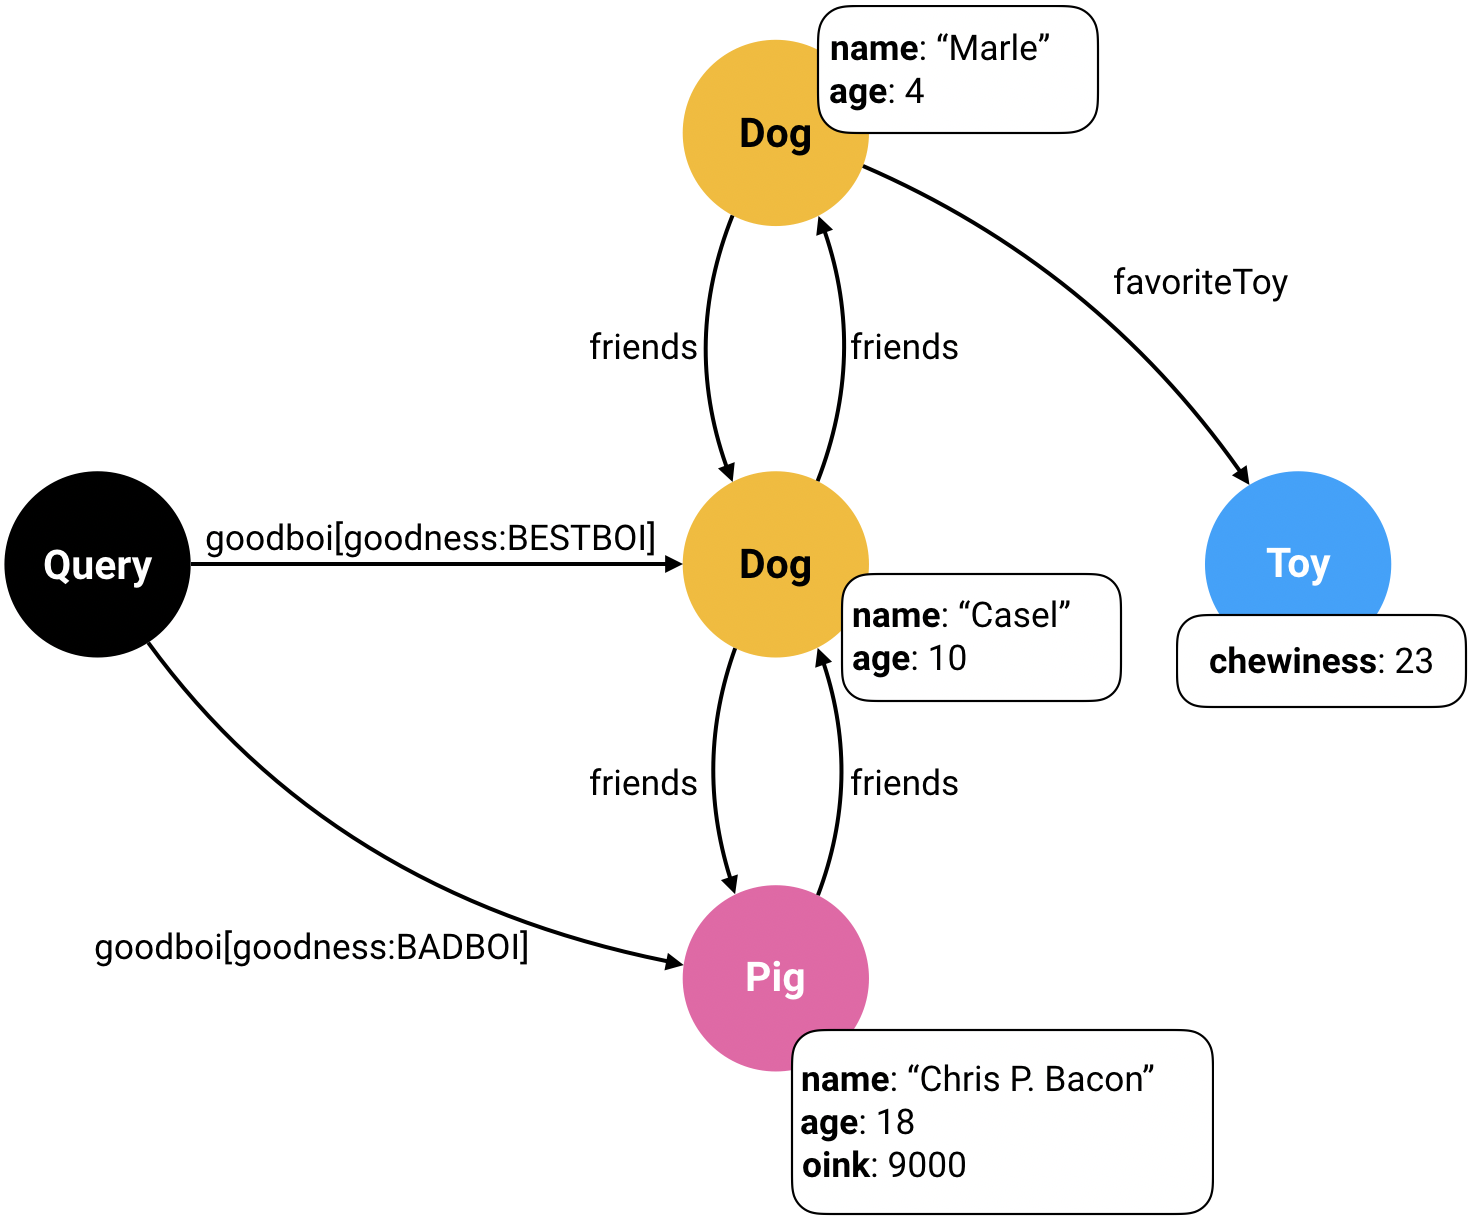
\includegraphics[scale=0.23]{imgs/graph.png}
    \caption{Example of GraphQL graph \et{favourite $\rightarrow$ favorite}}
    \label{fig:graph_ex}
\end{figure}

Finally, now that we have defined our type system and data, our developers can proceed to query it.

\subsection*{GraphQL Query and Response}

As previously mentioned, the queries we perform over our system must be over the types and fields defined in the schema. Every query must start by requesting information from the \texttt{Query} type. That means that, in our setting, queries must all start with the \texttt{goodness} or \texttt{search} fields.

In figure \ref{fig:qres_ex}, we can see a query where we asking for all the friends of the \texttt{BESTBOI} in our system. For each friend we ask for their \texttt{name}. The query can be further specified, using fragments, and say that for the \texttt{Dog} friends we want to know their toy's \texttt{chewiness} and for the \texttt{Pig} friends, their \texttt{oink} level. We rename this last selection to \texttt{loudness}. As we can see from this example, queries in GraphQL have a tree structure similar to JSON.

If we evaluate this query in the graph depicted in \ref{fig:graph_ex}, we would get the response shown in figure \ref{fig:qres_ex}. This response was obtained by navigating the graph and collecting the information contained in each of the relevant nodes. It is easy to see that the response has a structure very similar to the query's.

\begin{figure*}
\centering
\begin{subfigure}{.5\textwidth}
\begin{minted}[fontsize=\footnotesize, escapeinside=||,mathescape=true]{js}
query {
    goodboi(goodnessLevel: BESTBOI) {
        name
        friends {
            name
            |$\ldots$| on Dog {
                favoriteToy {
                    chewiness
                }
            }
            |$\ldots$| on Pig {
                loudness:oink
            }
        }
    }
}
\end{minted}
\label{fig:query_ex}
\end{subfigure}%
\begin{subfigure}{.5\textwidth}
\begin{minted}[fontsize=\footnotesize]{json}
{
    "goodboi": {
        "name":"Casel",
        "friends":[
            {
                "name": "Marle",
                "favoriteToy": {
                    "chewiness": 23
                }
            },
            {
                "name": "Chris P. Bacon",
                "loudness": 9000
            }
        ]
    }
}
\end{minted}
\label{fig:response_ex}
\end{subfigure}

\caption{Example of GraphQL query (left) and its response (right).}
\label{fig:qres_ex}
\end{figure*}

If we wanted to ask another the same query but now without the friends' names, we would only have to remove the \texttt{name} field and \textit{voilà}, that's it. We use the same endpoint as before and the GraphQL service handles the resolution of our fields.

With this we conclude our brief introduction to GraphQL and we can now move onto the formalization. We will come back to this example throughout the rest of the paper, illustrating how it can be replicated in our system.

The key points to take from our example are ...
